\documentclass[11pt,]{article}
\usepackage[left=1in,top=1in,right=1in,bottom=1in]{geometry}
\newcommand*{\authorfont}{\fontfamily{phv}\selectfont}
\usepackage[]{mathpazo}


  \usepackage[T1]{fontenc}
  \usepackage[utf8]{inputenc}



\usepackage{abstract}
\renewcommand{\abstractname}{}    % clear the title
\renewcommand{\absnamepos}{empty} % originally center

\renewenvironment{abstract}
 {{%
    \setlength{\leftmargin}{0mm}
    \setlength{\rightmargin}{\leftmargin}%
  }%
  \relax}
 {\endlist}

\makeatletter
\def\@maketitle{%
  \newpage
%  \null
%  \vskip 2em%
%  \begin{center}%
  \let \footnote \thanks
    {\fontsize{18}{20}\selectfont\raggedright  \setlength{\parindent}{0pt} \@title \par}%
}
%\fi
\makeatother




\setcounter{secnumdepth}{3}

\usepackage{color}
\usepackage{fancyvrb}
\newcommand{\VerbBar}{|}
\newcommand{\VERB}{\Verb[commandchars=\\\{\}]}
\DefineVerbatimEnvironment{Highlighting}{Verbatim}{commandchars=\\\{\}}
% Add ',fontsize=\small' for more characters per line
\usepackage{framed}
\definecolor{shadecolor}{RGB}{248,248,248}
\newenvironment{Shaded}{\begin{snugshade}}{\end{snugshade}}
\newcommand{\KeywordTok}[1]{\textcolor[rgb]{0.13,0.29,0.53}{\textbf{#1}}}
\newcommand{\DataTypeTok}[1]{\textcolor[rgb]{0.13,0.29,0.53}{#1}}
\newcommand{\DecValTok}[1]{\textcolor[rgb]{0.00,0.00,0.81}{#1}}
\newcommand{\BaseNTok}[1]{\textcolor[rgb]{0.00,0.00,0.81}{#1}}
\newcommand{\FloatTok}[1]{\textcolor[rgb]{0.00,0.00,0.81}{#1}}
\newcommand{\ConstantTok}[1]{\textcolor[rgb]{0.00,0.00,0.00}{#1}}
\newcommand{\CharTok}[1]{\textcolor[rgb]{0.31,0.60,0.02}{#1}}
\newcommand{\SpecialCharTok}[1]{\textcolor[rgb]{0.00,0.00,0.00}{#1}}
\newcommand{\StringTok}[1]{\textcolor[rgb]{0.31,0.60,0.02}{#1}}
\newcommand{\VerbatimStringTok}[1]{\textcolor[rgb]{0.31,0.60,0.02}{#1}}
\newcommand{\SpecialStringTok}[1]{\textcolor[rgb]{0.31,0.60,0.02}{#1}}
\newcommand{\ImportTok}[1]{#1}
\newcommand{\CommentTok}[1]{\textcolor[rgb]{0.56,0.35,0.01}{\textit{#1}}}
\newcommand{\DocumentationTok}[1]{\textcolor[rgb]{0.56,0.35,0.01}{\textbf{\textit{#1}}}}
\newcommand{\AnnotationTok}[1]{\textcolor[rgb]{0.56,0.35,0.01}{\textbf{\textit{#1}}}}
\newcommand{\CommentVarTok}[1]{\textcolor[rgb]{0.56,0.35,0.01}{\textbf{\textit{#1}}}}
\newcommand{\OtherTok}[1]{\textcolor[rgb]{0.56,0.35,0.01}{#1}}
\newcommand{\FunctionTok}[1]{\textcolor[rgb]{0.00,0.00,0.00}{#1}}
\newcommand{\VariableTok}[1]{\textcolor[rgb]{0.00,0.00,0.00}{#1}}
\newcommand{\ControlFlowTok}[1]{\textcolor[rgb]{0.13,0.29,0.53}{\textbf{#1}}}
\newcommand{\OperatorTok}[1]{\textcolor[rgb]{0.81,0.36,0.00}{\textbf{#1}}}
\newcommand{\BuiltInTok}[1]{#1}
\newcommand{\ExtensionTok}[1]{#1}
\newcommand{\PreprocessorTok}[1]{\textcolor[rgb]{0.56,0.35,0.01}{\textit{#1}}}
\newcommand{\AttributeTok}[1]{\textcolor[rgb]{0.77,0.63,0.00}{#1}}
\newcommand{\RegionMarkerTok}[1]{#1}
\newcommand{\InformationTok}[1]{\textcolor[rgb]{0.56,0.35,0.01}{\textbf{\textit{#1}}}}
\newcommand{\WarningTok}[1]{\textcolor[rgb]{0.56,0.35,0.01}{\textbf{\textit{#1}}}}
\newcommand{\AlertTok}[1]{\textcolor[rgb]{0.94,0.16,0.16}{#1}}
\newcommand{\ErrorTok}[1]{\textcolor[rgb]{0.64,0.00,0.00}{\textbf{#1}}}
\newcommand{\NormalTok}[1]{#1}

\usepackage{graphicx,grffile}
\makeatletter
\def\maxwidth{\ifdim\Gin@nat@width>\linewidth\linewidth\else\Gin@nat@width\fi}
\def\maxheight{\ifdim\Gin@nat@height>\textheight\textheight\else\Gin@nat@height\fi}
\makeatother
% Scale images if necessary, so that they will not overflow the page
% margins by default, and it is still possible to overwrite the defaults
% using explicit options in \includegraphics[width, height, ...]{}
\setkeys{Gin}{width=\maxwidth,height=\maxheight,keepaspectratio}

\title{Análisis Geostadístico de la Variabilidad en la precipitación pluvial en
República Dominicana.  }



\author{\Large Aleira Del Jesús, Grace Soriano, Wilnellia Fabián\vspace{0.05in} \newline\normalsize\emph{Estudiantes de la Mestría en Teledetección y Ciencias de la Información
Geográfica, Universidad Autónoma de Santo Domingo (UASD).}  }


\date{}

\usepackage{titlesec}

\titleformat*{\section}{\normalsize\bfseries}
\titleformat*{\subsection}{\normalsize\itshape}
\titleformat*{\subsubsection}{\normalsize\itshape}
\titleformat*{\paragraph}{\normalsize\itshape}
\titleformat*{\subparagraph}{\normalsize\itshape}

\titlespacing{\section}
{0pt}{36pt}{0pt}
\titlespacing{\subsection}
{0pt}{36pt}{0pt}
\titlespacing{\subsubsection}
{0pt}{36pt}{0pt}





\newtheorem{hypothesis}{Hypothesis}
\usepackage{setspace}

\makeatletter
\@ifpackageloaded{hyperref}{}{%
\ifxetex
  \PassOptionsToPackage{hyphens}{url}\usepackage[setpagesize=false, % page size defined by xetex
              unicode=false, % unicode breaks when used with xetex
              xetex]{hyperref}
\else
  \PassOptionsToPackage{hyphens}{url}\usepackage[unicode=true]{hyperref}
\fi
}

\@ifpackageloaded{color}{
    \PassOptionsToPackage{usenames,dvipsnames}{color}
}{%
    \usepackage[usenames,dvipsnames]{color}
}
\makeatother
\hypersetup{breaklinks=true,
            bookmarks=true,
            pdfauthor={Aleira Del Jesús, Grace Soriano, Wilnellia Fabián (Estudiantes de la Mestría en Teledetección y Ciencias de la Información
Geográfica, Universidad Autónoma de Santo Domingo (UASD).)},
             pdfkeywords = {Variabilidad Pluviométrica, Precipitación,Clima},  
            pdftitle={Análisis Geostadístico de la Variabilidad en la precipitación pluvial en
República Dominicana.},
            colorlinks=true,
            citecolor=blue,
            urlcolor=blue,
            linkcolor=magenta,
            pdfborder={0 0 0}}
\urlstyle{same}  % don't use monospace font for urls

% set default figure placement to htbp
\makeatletter
\def\fps@figure{htbp}
\makeatother

\usepackage{pdflscape} \newcommand{\blandscape}{\begin{landscape}}
\newcommand{\elandscape}{\end{landscape}}


% add tightlist ----------
\providecommand{\tightlist}{%
\setlength{\itemsep}{0pt}\setlength{\parskip}{0pt}}

\begin{document}
	
% \pagenumbering{arabic}% resets `page` counter to 1 
%
% \maketitle

{% \usefont{T1}{pnc}{m}{n}
\setlength{\parindent}{0pt}
\thispagestyle{plain}
{\fontsize{18}{20}\selectfont\raggedright 
\maketitle  % title \par  

}

{
   \vskip 13.5pt\relax \normalsize\fontsize{11}{12} 
\textbf{\authorfont Aleira Del Jesús, Grace Soriano, Wilnellia Fabián} \hskip 15pt \emph{\small Estudiantes de la Mestría en Teledetección y Ciencias de la Información
Geográfica, Universidad Autónoma de Santo Domingo (UASD).}   

}

}








\begin{abstract}

    \hbox{\vrule height .2pt width 39.14pc}

    \vskip 8.5pt % \small 

\noindent Resumen. El clima anualmente se ve afectado por los cambios que se
producen en la superficie terrestre. Estos se los podemos atribuir,
tanto al impacto humano como a la naturaleza. La precipitación es una
parte muy importante de la composición del ciclo hidrológico, es por
ello, que en la actualidad existe gran interés por conocer los factores
que controlan el clima, en virtud del incremento en los desastres
naturales que afectan la población. Por lo que, con la finalidad de
poder obtener conocimiento sobre el valor trascendental de los cambios
observados en las provincias de la República Dominicana, se analizó la
variabilidad pluviométrica de la precipitación, correspondiente al año
1994.


\vskip 8.5pt \noindent \emph{Keywords}: Variabilidad Pluviométrica, Precipitación,Clima \par

    \hbox{\vrule height .2pt width 39.14pc}



\end{abstract}


\vskip 6.5pt


\noindent  \section{Introducción}\label{introducciuxf3n}

La Finalidad de realizar este proyecto, es lograr conocer la
variabilidad en la precipitación pluvial en la República Dominicana,
específicamente para el año 1994. Con el objetivo de conocer la cantidad
de lluvia en cada provincia durante ese período, dicha información nos
permite identificar las zonas vulnerables a inundaciones o deslizamiento
ante un fenómeno atmoférico.

Desarrollaremos nuestro trabajo mediante el Análisis Geoestadístico, el
cual está basado en el hecho de que los datos esten correlacionados
espacialmente, o sea, que un dato va a estar relacionado con otros datos
cercanos, por lo que, a medida que nos alejamos del dato, esta
dependencia va perdiendo fuerza. En ese mismo sentido, podemos decir,
que la geoestadística, es una ciencia aplicada, la cual estudia las
variables que se distribuyen espacialmente y toma muestras que son
referencias del fenómeno objeto de estudio.

Según artículo publicado por ({\textbf{???}})\{garcía2009variabilidad,
dice que los cambios climáticos anuales y de un periodo a otro se pueden
atribuir tanto a la variabilidad natural del clima como al cambio
ocasionado por las actividades antropogénicas, por lo que, es importante
conocer las zonas de nuestro país que son vulnerables a esos cambios.

\section{Metodología}\label{metodologuxeda}

-Utilizamos el entorno de programación estadística R y el entorno de
desarrollo integrado RStudio para el progreso de nuestro proyecto.

-Clonamos desde el Github la carpeta de ``mi proyecto'', la cual
contiene los datos correspondientes para realizar los análisis
espaciales.

-Los datos fueron suministrados por el profesor, el cual los obtuvo a
través de la Oficina Nacional de Meteorrologia (ONAMET), que es el ente
encargado de regulador la investigación y producción de la información
meteorológica en el país.

-Haciendo una evaluación de los datos proporcionados, decidimos trabajar
con el año 1994, ya que posee pocos datos perdidos, lo que a nuestro
entender arrojaría buenos resultados.

-Realizamos una serie de cálculos previos, a efectuar la interpolación
por Kriging oridinario, como es, el cálculo de los Variogramas
Muestrales y de los Variogramas Modelos, para luego obtener un resultado
respecto a los datos analizados.

-Los datos de las precipitaciones del año 1994, fueron extraídos de la
siguiente tabla:

\begin{Shaded}
\begin{Highlighting}[]
\NormalTok{prep }\OperatorTok\StringTok{ }\KeywordTok{st_drop_geometry}\NormalTok{()}
\end{Highlighting}
\end{Shaded}

\begin{verbatim}
##              Estación  a1979  a1980  a1981   a1982   a1983  a1984   a1985
## 1            Barahona 1740.0 1053.6 1435.3  815.30 1183.00  584.1  997.80
## 2           Bayaguana 2794.3 1761.5 2412.4 1758.60 1857.10 1645.6 1928.30
## 3             Cabrera 2035.0 1276.8     NA 2136.90 1703.80 1888.7 1557.10
## 4           Constanza 1652.1 1166.9 1343.3  921.20  828.40     NA  892.80
## 5    Gaspar Hernández     NA 1443.8 2174.9 1844.10 1688.80 2208.8 1895.50
## 6         Hondo Valle 1823.6 1778.2 2203.7 1709.90 1841.30 1796.6 1309.50
## 7              Jimaní 1060.7  639.1  960.2  507.50  610.70  641.5  689.60
## 8            La Unión 1781.5 1630.6 2304.4 1413.10 1288.40 1499.4 1157.10
## 9             La Vega 1833.5 1304.3 1993.7 1483.20 1353.90 1550.1 1084.90
## 10       Las Américas 1958.4  958.7 1513.4  787.40  975.50  954.9 1398.20
## 11               Moca 1571.2 1169.8 1493.6 1426.30  975.40 1256.8 1183.60
## 12       Monte Cristi  835.0  991.6  642.7  439.20  447.30  579.4  683.70
## 13    Padre Las Casas 1345.0  845.4  743.0  567.90  627.30  824.6  598.90
## 14               Polo 3054.2 1523.2 2124.8 1687.60 1320.20 1429.9 2227.30
## 15         Punta Cana 1449.5 1078.2 1663.1 1224.00  920.70 1095.8  964.60
## 16      Rancho Arriba     NA  453.8 1760.0 1376.35 1230.35 1583.1 1549.95
## 17       Río San Juan 3621.0 1627.2 3004.5 2651.30 2300.90 2350.1 1993.50
## 18   Sabana de la Mar 3621.0 1627.2 3004.5 2651.30 2300.90 2350.1 1993.50
## 19            Salcedo     NA     NA 1546.9 1419.70 1195.10 1278.4 1266.10
## 20             Samaná 3106.2 1859.4 2449.0 2515.00 2201.40 2362.9 1959.30
## 21      San Cristóbal 2925.8  938.1 1184.9 1316.60 1234.30 1384.7      NA
## 22           Santiago 1550.8  934.3 1326.9  950.60  913.60 1268.2  847.20
## 23 Santiago Rodríguez 1407.0 1206.7  968.0 1024.40 1012.70 1189.3 1252.10
## 24      Santo Domingo 2232.6 1257.8 1623.2 1278.70 1355.00 1331.5 1749.30
## 25      Villa Vázquez     NA 1072.3  903.2  418.80  393.10  687.8  489.80
##      a1986   a1987  a1988    a1989   a1990  a1991    a1992  a1993   a1994
## 1  1080.00 1423.90  704.7 1011.600 1075.20  983.1 1112.500  968.5 1622.40
## 2  2182.20 2273.50 1813.2 1730.600 1823.40 1850.3 1765.700 1606.2 1892.80
## 3  1597.00 2059.70     NA 1176.900 1183.40  957.6       NA     NA      NA
## 4   715.80  786.90  837.7  671.500  875.35     NA  858.600  858.6  900.70
## 5  2874.70 2360.80 1426.3 1214.200 1530.70     NA 1257.500 1345.3 1824.90
## 6  1589.70 1778.80 1766.5 1722.800 1596.10 1088.4 1731.000 1887.0 1772.00
## 7   802.40  648.90  521.0  680.700  880.00  311.6  809.200  472.9  840.20
## 8  1313.10 1786.50 1888.8 1222.800 1808.00 1250.4 1555.200 1484.8 1035.90
## 9  1767.10 1663.20 1934.9 1192.400 1664.40 1146.4 1565.600 1855.4 1455.70
## 10 1419.00 1866.40 1620.5 1151.700      NA  997.0       NA     NA      NA
## 11 1136.00 1257.00 1513.5 1034.900 1639.50  780.3  935.950 1158.4 1182.10
## 12  511.60  870.00  670.5  454.500  679.90     NA  420.400  466.8  650.05
## 13  816.80  873.30  764.0  683.200  785.40  523.0  734.300  763.8  750.40
## 14  703.20 2203.70 2050.9 1744.792 2077.10     NA 1929.635     NA 1646.90
## 15 1145.75 1297.70 1236.0  746.900  917.60     NA 1190.600  821.1 1119.70
## 16 1290.50 1639.60 2062.2 1494.300 1608.40 1217.6 1858.200 1651.9 1391.00
## 17 2529.40 2872.90 2670.0 2072.000 2261.20     NA 2429.200 2047.4 1879.70
## 18 2529.40 2872.90 2670.0       NA 2248.70 1890.7 2429.200 2034.9 1879.70
## 19 1386.20 1564.40 2001.3 1101.400 1462.80  941.0 1272.200 1095.3 1042.10
## 20 2880.90 2286.60 2613.5 2335.100 1861.50     NA 2087.200 2244.4 1793.00
## 21      NA 1481.90 1768.2 1420.600 1371.90 1286.6 1759.600 1772.3 1933.70
## 22  870.60 1424.70 1288.4  724.000 1104.40  496.5 1045.300  953.4  736.90
## 23  622.90 1269.25 1186.6 1003.100 1175.30     NA 1035.700 1463.7  978.30
## 24 1815.00 2003.10 2024.6 1613.600 1482.30     NA 1224.800 1478.4 1219.50
## 25  405.40  735.80  663.8  499.500  512.80     NA  508.300  677.0  955.90
##      a1995   a1996   a1997   a1998   a1999  a2000   a2001  a2002   a2003
## 1   956.00  965.65  662.60  684.60  662.70  600.0  600.00  997.6  942.60
## 2  1360.10 1867.70 1618.60 2156.60 1712.50 1868.5 1796.10 1658.0 2117.30
## 3       NA      NA      NA      NA      NA 1538.6 1852.90  946.9 1810.95
## 4   839.40 1167.30  525.10 1492.70 1077.80  951.3  787.10  959.2 1084.10
## 5  1665.45 2656.80  984.80 2147.90 1791.90 1716.9 2178.80 1093.4 2058.50
## 6  1288.30 1447.90  912.65 1813.90 1762.20 2285.9 1604.30 1477.4 1628.10
## 7   909.00  816.20  358.20  824.10 1037.00  833.9  488.40  510.1  656.70
## 8   877.70 1980.50  554.20 1744.10 1314.30 1148.5 1360.50  972.1 1802.00
## 9  1175.40 1772.50 1018.80 1549.60 1817.90 1368.6 1522.00 1200.7 2290.60
## 10 1017.50 1019.60  651.20 1218.60 1125.90  809.7  747.60  933.4 1083.60
## 11 1026.10 1345.70  646.20 1036.40 1270.00  852.4 1045.20  677.3 1734.60
## 12      NA  787.00  649.30  929.40  714.10  818.3      NA  581.6 1058.10
## 13  634.30  794.50  374.00 1084.80  696.70  431.0  543.70  569.2  771.10
## 14 1451.10 1688.90 1486.40 1641.50 1151.40     NA 1228.10 1602.5 1777.80
## 15 1029.10 1483.60 1072.30 1284.90  875.20  994.7 1106.50  943.4 1220.10
## 16 1361.10 2043.40  698.70 1988.20 1690.15 1364.8 1294.75 1477.3 1856.30
## 17 2394.70 2729.90 1752.30 3011.30 2669.10 1555.7 1913.60 1594.6 1894.60
## 18 2394.70 4108.40 1752.30 3011.30 2669.10 1555.7 1913.60 1594.6 1888.60
## 19 1218.00      NA      NA 1580.55 1875.50 1235.8 1735.30 1189.1 1401.30
## 20 2020.90 3299.90 1559.00 2550.30 2177.40 1316.5 2011.70 1815.3 2061.00
## 21 1849.20 1824.40 1108.10 1878.70 1193.80 1156.2 1085.30 1498.4 1695.60
## 22  652.80  992.20  398.00      NA      NA  744.0  764.20  528.2 1518.90
## 23 1188.30 1245.00 1033.60 1265.80 1392.20  925.4 1390.50 1157.3 1485.40
## 24 1620.50 1369.40 1271.30 1987.10 1529.50 1241.1 1261.10 1208.8 1561.80
## 25  820.40  787.00  649.30  929.40  714.10  818.3  776.20  581.6 1058.10
##      a2004    a2005   a2006   a2007   a2008   a2009  a2010  a2011  a2012
## 1   972.60 1274.600 1118.40 1531.30 1136.80  583.30 1036.3 1280.2 1726.3
## 2  1554.20 2102.800 2097.10 2137.60 1831.20 1607.90 1881.6 1849.9 2350.8
## 3  2053.30 1451.100 1957.90      NA      NA      NA 2411.4 1920.1 2821.3
## 4   985.90 1245.200 1162.20 1661.40 1072.90  902.80 1024.5 1008.2 1188.1
## 5  1906.80 2001.850 1992.00 3282.65 1866.30 2386.10 2639.2 1727.2 2524.0
## 6  1617.70 1554.650 1487.15 1487.15 1399.15 1461.90 2005.6 1309.0 1736.8
## 7   866.90  929.300  963.90 1084.00  751.10  694.90  807.1  879.5 1037.3
## 8  2550.10 2034.300 2106.60 2764.80 1536.30 1605.80 2255.6 1719.2 2484.3
## 9  1825.70 1245.200 1162.20 1661.40 1072.90 2867.40 1486.4 1434.1 2204.7
## 10 1338.90 1744.600 1141.70 1457.50 1718.40 1369.10 2422.4 1885.5 1658.7
## 11 1541.20 1916.600 1392.90 2429.80 1144.30 1342.30 1360.9 1291.5 1799.5
## 12  896.20  912.600  766.70 1027.70  560.50  525.10 1096.9  424.1 1351.4
## 13  691.35  914.500  636.15  636.15  659.10  782.00  684.9  868.6 1001.5
## 14 1646.90 2145.701 1734.00 2417.30 2129.60 1633.50 2373.4 2173.5 2726.4
## 15 1229.40 1125.200 1323.30 1356.10 1490.80 1292.60 1305.0 1577.6 1555.6
## 16 1831.90 1835.600 1521.80 2467.30 2112.10 1582.40 1683.2 1042.4 1918.3
## 17 2053.30 1451.100 2465.30 2763.50 2376.00 2350.50 2101.3 1325.9 1681.4
## 18 2053.30 2280.400 1788.80 2165.60 1688.00 2684.15 2695.0 2520.4 2599.0
## 19 2014.00 2135.700 1682.30 2363.20 1611.70 1627.60 1884.3 2100.3 1700.9
## 20 1891.20 2382.200 2135.70 1682.30 2363.20 1611.70 1627.6 1884.3 2100.3
## 21 1685.90 1641.700 1361.60 1689.00 1704.20 1613.70 1361.8 1417.4 1885.3
## 22 1394.70 1411.600 1209.90 1992.30  878.30 1170.90 1499.7 1353.1 1687.2
## 23 1104.40 1317.500 1528.10 1818.10 1021.80 1445.20 1421.1 1207.6 1434.7
## 24 1509.40 1505.900 1209.70 1916.00 2098.90 1559.20 1876.3 2118.8 1554.0
## 25  896.20  912.600  766.70 1209.10  721.60  866.30  869.2  654.5  962.8
##     a2013  a2014
## 1   576.2  845.9
## 2  2108.0 1505.6
## 3      NA 1975.6
## 4  1016.3  764.1
## 5  1448.2 1928.7
## 6  1390.2  908.9
## 7   292.9  502.0
## 8  1299.2 1741.5
## 9  1227.0 1812.5
## 10 1039.6  909.4
## 11 1384.2 1094.2
## 12  425.7  603.7
## 13  938.5  872.3
## 14 2058.5 1798.4
## 15 1027.1  876.8
## 16  868.8 1410.3
## 17  890.1 1251.2
## 18 2197.6 1499.0
## 19 1877.1 1723.4
## 20 1700.9 1931.3
## 21 1188.4 1352.8
## 22 1139.4  991.0
## 23 1096.4 1287.4
## 24 1262.9 1242.8
## 25  587.0 1040.0
\end{verbatim}

\section{Resultados}\label{resultados}

En el análisis realizado de los datos de precipitación, podemos
visualizar mediante el variograma que los mismos tienen un incremento
gradual de la semivarianza hasta que se alcanza la meseta en el rango,
por lo que, la semivarianza inicia en cero o cercana a éste. Por ende,
existe autocorrelación espacial.

En el histograma visualiza que los datos están sesgado hacia la derecha
con relación a su distribución. En ese mismo orden, podemos resaltar que
en el país tenemos 25 observatorios, de los cuales para ese año sólo 2
tienen datos no encontrados.

El mapa generado nos muestra que el valor de la precipatación para ese
año oscila entre 700-1000, notándose que las provincias donde tuvieron
una precipitación mayor durante ese período fueron las que poseen el
color azul mas intenso, algunas de ellas son: Sánchez Ramírez,
Espaillat, Monte Plata, Distrito Nacional, Hato Mayor y San Pedro de
Macoris, y las que poseen un color azul menos intenso, indican que la
precipitación fue menor, pudiendo mencionar dentro de esta a Monte
Cristi, Santiago, Azua y Pedernales, entre otras.

\begin{Shaded}
\begin{Highlighting}[]
\CommentTok{#ESTADÍSTICOS BÁSICOS PARA EL AÑO 1994.}

\KeywordTok{nrow}\NormalTok{(preputm)}
\end{Highlighting}
\end{Shaded}

\begin{verbatim}
## [1] 25
\end{verbatim}

\begin{Shaded}
\begin{Highlighting}[]
\KeywordTok{summary}\NormalTok{(preputm}\OperatorTok{$}\NormalTok{a1994)}
\end{Highlighting}
\end{Shaded}

\begin{verbatim}
##    Min. 1st Qu.  Median    Mean 3rd Qu.    Max.    NA's 
##   650.0   967.1  1219.5  1326.2  1782.5  1933.7       2
\end{verbatim}

\begin{Shaded}
\begin{Highlighting}[]
\KeywordTok{hist}\NormalTok{(preputm}\OperatorTok{$}\NormalTok{a1994)}
\end{Highlighting}
\end{Shaded}

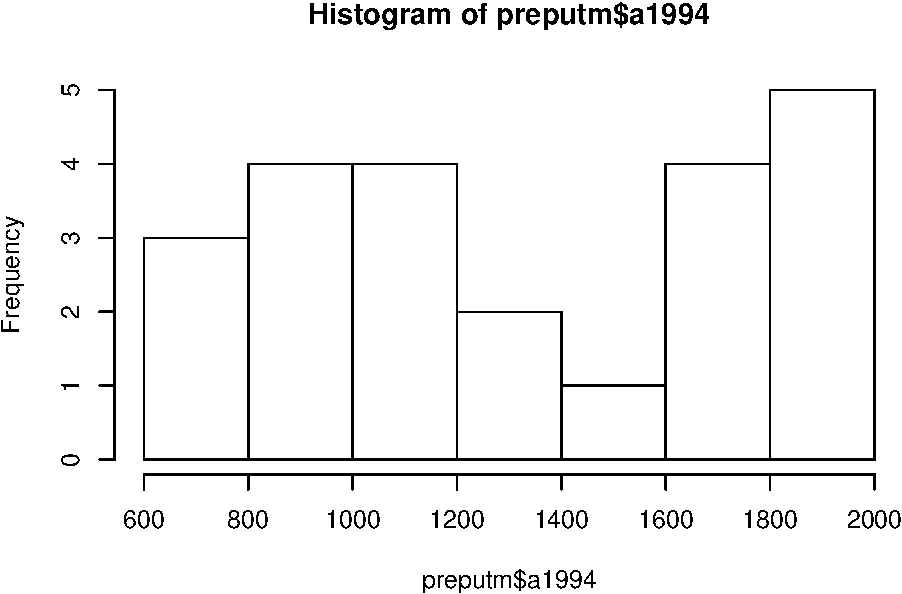
\includegraphics{proyecto_files/figure-latex/unnamed-chunk-3-1.pdf}

\begin{Shaded}
\begin{Highlighting}[]
\KeywordTok{hist}\NormalTok{(}\KeywordTok{log}\NormalTok{(preputm}\OperatorTok{$}\NormalTok{a1994))}
\end{Highlighting}
\end{Shaded}

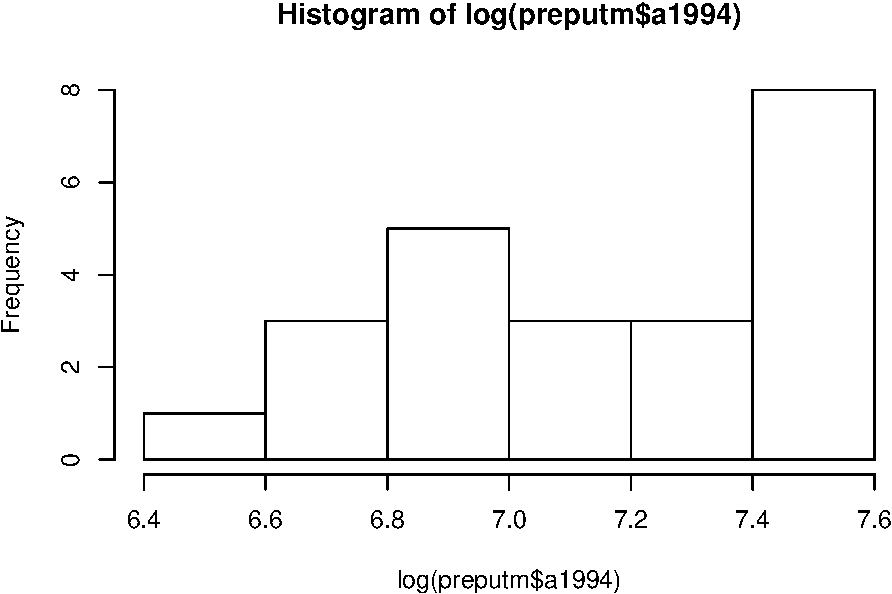
\includegraphics{proyecto_files/figure-latex/unnamed-chunk-3-2.pdf}

\begin{Shaded}
\begin{Highlighting}[]
\KeywordTok{shapiro.test}\NormalTok{(preputm}\OperatorTok{$}\NormalTok{a1994)}
\end{Highlighting}
\end{Shaded}

\begin{verbatim}
## 
##  Shapiro-Wilk normality test
## 
## data:  preputm$a1994
## W = 0.9062, p-value = 0.03399
\end{verbatim}

\begin{Shaded}
\begin{Highlighting}[]
\KeywordTok{shapiro.test}\NormalTok{(}\KeywordTok{log}\NormalTok{(prep}\OperatorTok{$}\NormalTok{a1994))}
\end{Highlighting}
\end{Shaded}

\begin{verbatim}
## 
##  Shapiro-Wilk normality test
## 
## data:  log(prep$a1994)
## W = 0.91635, p-value = 0.05567
\end{verbatim}

\section{Discusión o Conclusiones}\label{discusiuxf3n-o-conclusiones}

A partir de los resultados obtenidos para el año 1994, concluimos que
los datos visualizados a través de los variogramas muestrales generados
del ajuste del variograma modelo, indican que tienen un incremento
gradual hasta alcanzar el rango, por lo que podemos concluir que
nuestros datos arrojan un 95\% de confianza, ya que p-valor
\textgreater{} 0.05.

Se llevó acabo la realización del Análisis Geoestadístico, con el
objetivo principal de emplear la técnica Kriging Ordinario, para así
poder obtener una predicción de los valores desconocidos de la
precipitación correspodiente al año 1994, con la finalidad de poder
identificar las provincias que son vulnerables a los fenómenos
atmoféricos. En aras, de que el país pueda establecer las medidas
necesarias ante un evento inesperado.

\section{\texorpdfstring{\emph{Script}
reproducible}{Script reproducible}}\label{script-reproducible}

\begin{Shaded}
\begin{Highlighting}[]
\KeywordTok{library}\NormalTok{(sf)}
\KeywordTok{library}\NormalTok{(tidyverse)}
\KeywordTok{library}\NormalTok{(spdep)}
\KeywordTok{library}\NormalTok{(lmtest)}
\KeywordTok{library}\NormalTok{(tmap)}
\KeywordTok{library}\NormalTok{(RColorBrewer)}
\KeywordTok{library}\NormalTok{(ggplot2)}
\KeywordTok{library}\NormalTok{(gstat)}
\KeywordTok{library}\NormalTok{(stars)}

\CommentTok{#Cargamos los datos correspondientes a las provincias y los observatorios}
\NormalTok{rutaprep <-}\StringTok{ 'data/onamet_prec_anual_sf.gpkg'}
\NormalTok{rutadiv <-}\StringTok{ 'data/divisionRD.gpkg'}
\KeywordTok{st_layers}\NormalTok{(rutaprep)}
\end{Highlighting}
\end{Shaded}

\begin{verbatim}
## Driver: GPKG 
## Available layers:
##             layer_name geometry_type features fields
## 1 onamet_prec_anual_sf         Point       25     37
\end{verbatim}

\begin{Shaded}
\begin{Highlighting}[]
\NormalTok{prep <-}\StringTok{ }\KeywordTok{st_read}\NormalTok{(rutaprep)}
\end{Highlighting}
\end{Shaded}

\begin{verbatim}
## Reading layer `onamet_prec_anual_sf' from data source `/home/wilne/unidad-0-asignacion-99-mi-proyecto-wilnellia/data/onamet_prec_anual_sf.gpkg' using driver `GPKG'
## Simple feature collection with 25 features and 37 fields
## geometry type:  POINT
## dimension:      XY
## bbox:           xmin: -71.7 ymin: 18.067 xmax: -68.367 ymax: 19.85
## epsg (SRID):    4326
## proj4string:    +proj=longlat +datum=WGS84 +no_defs
\end{verbatim}

\begin{Shaded}
\begin{Highlighting}[]
\NormalTok{prep}
\end{Highlighting}
\end{Shaded}

\begin{verbatim}
## Simple feature collection with 25 features and 37 fields
## geometry type:  POINT
## dimension:      XY
## bbox:           xmin: -71.7 ymin: 18.067 xmax: -68.367 ymax: 19.85
## epsg (SRID):    4326
## proj4string:    +proj=longlat +datum=WGS84 +no_defs
## First 10 features:
##            Estación  a1979  a1980  a1981  a1982  a1983  a1984  a1985
## 1          Barahona 1740.0 1053.6 1435.3  815.3 1183.0  584.1  997.8
## 2         Bayaguana 2794.3 1761.5 2412.4 1758.6 1857.1 1645.6 1928.3
## 3           Cabrera 2035.0 1276.8     NA 2136.9 1703.8 1888.7 1557.1
## 4         Constanza 1652.1 1166.9 1343.3  921.2  828.4     NA  892.8
## 5  Gaspar Hernández     NA 1443.8 2174.9 1844.1 1688.8 2208.8 1895.5
## 6       Hondo Valle 1823.6 1778.2 2203.7 1709.9 1841.3 1796.6 1309.5
## 7            Jimaní 1060.7  639.1  960.2  507.5  610.7  641.5  689.6
## 8          La Unión 1781.5 1630.6 2304.4 1413.1 1288.4 1499.4 1157.1
## 9           La Vega 1833.5 1304.3 1993.7 1483.2 1353.9 1550.1 1084.9
## 10     Las Américas 1958.4  958.7 1513.4  787.4  975.5  954.9 1398.2
##     a1986  a1987  a1988  a1989   a1990  a1991  a1992  a1993  a1994   a1995
## 1  1080.0 1423.9  704.7 1011.6 1075.20  983.1 1112.5  968.5 1622.4  956.00
## 2  2182.2 2273.5 1813.2 1730.6 1823.40 1850.3 1765.7 1606.2 1892.8 1360.10
## 3  1597.0 2059.7     NA 1176.9 1183.40  957.6     NA     NA     NA      NA
## 4   715.8  786.9  837.7  671.5  875.35     NA  858.6  858.6  900.7  839.40
## 5  2874.7 2360.8 1426.3 1214.2 1530.70     NA 1257.5 1345.3 1824.9 1665.45
## 6  1589.7 1778.8 1766.5 1722.8 1596.10 1088.4 1731.0 1887.0 1772.0 1288.30
## 7   802.4  648.9  521.0  680.7  880.00  311.6  809.2  472.9  840.2  909.00
## 8  1313.1 1786.5 1888.8 1222.8 1808.00 1250.4 1555.2 1484.8 1035.9  877.70
## 9  1767.1 1663.2 1934.9 1192.4 1664.40 1146.4 1565.6 1855.4 1455.7 1175.40
## 10 1419.0 1866.4 1620.5 1151.7      NA  997.0     NA     NA     NA 1017.50
##      a1996   a1997  a1998  a1999  a2000  a2001  a2002   a2003  a2004
## 1   965.65  662.60  684.6  662.7  600.0  600.0  997.6  942.60  972.6
## 2  1867.70 1618.60 2156.6 1712.5 1868.5 1796.1 1658.0 2117.30 1554.2
## 3       NA      NA     NA     NA 1538.6 1852.9  946.9 1810.95 2053.3
## 4  1167.30  525.10 1492.7 1077.8  951.3  787.1  959.2 1084.10  985.9
## 5  2656.80  984.80 2147.9 1791.9 1716.9 2178.8 1093.4 2058.50 1906.8
## 6  1447.90  912.65 1813.9 1762.2 2285.9 1604.3 1477.4 1628.10 1617.7
## 7   816.20  358.20  824.1 1037.0  833.9  488.4  510.1  656.70  866.9
## 8  1980.50  554.20 1744.1 1314.3 1148.5 1360.5  972.1 1802.00 2550.1
## 9  1772.50 1018.80 1549.6 1817.9 1368.6 1522.0 1200.7 2290.60 1825.7
## 10 1019.60  651.20 1218.6 1125.9  809.7  747.6  933.4 1083.60 1338.9
##      a2005   a2006   a2007   a2008  a2009  a2010  a2011  a2012  a2013
## 1  1274.60 1118.40 1531.30 1136.80  583.3 1036.3 1280.2 1726.3  576.2
## 2  2102.80 2097.10 2137.60 1831.20 1607.9 1881.6 1849.9 2350.8 2108.0
## 3  1451.10 1957.90      NA      NA     NA 2411.4 1920.1 2821.3     NA
## 4  1245.20 1162.20 1661.40 1072.90  902.8 1024.5 1008.2 1188.1 1016.3
## 5  2001.85 1992.00 3282.65 1866.30 2386.1 2639.2 1727.2 2524.0 1448.2
## 6  1554.65 1487.15 1487.15 1399.15 1461.9 2005.6 1309.0 1736.8 1390.2
## 7   929.30  963.90 1084.00  751.10  694.9  807.1  879.5 1037.3  292.9
## 8  2034.30 2106.60 2764.80 1536.30 1605.8 2255.6 1719.2 2484.3 1299.2
## 9  1245.20 1162.20 1661.40 1072.90 2867.4 1486.4 1434.1 2204.7 1227.0
## 10 1744.60 1141.70 1457.50 1718.40 1369.1 2422.4 1885.5 1658.7 1039.6
##     a2014                    geom
## 1   845.9      POINT (-71.1 18.2)
## 2  1505.6 POINT (-69.63333 18.75)
## 3  1975.6    POINT (-69.9 19.633)
## 4   764.1      POINT (-70.7 18.9)
## 5  1928.7    POINT (-70.3 19.617)
## 6   908.9    POINT (-71.7 18.717)
## 7   502.0  POINT (-71.633 18.483)
## 8  1741.5    POINT (-70.55 19.75)
## 9  1812.5  POINT (-70.533 19.217)
## 10  909.4  POINT (-69.667 18.433)
\end{verbatim}

\begin{Shaded}
\begin{Highlighting}[]
\KeywordTok{st_layers}\NormalTok{(rutadiv)}
\end{Highlighting}
\end{Shaded}

\begin{verbatim}
## Driver: GPKG 
## Available layers:
##      layer_name geometry_type features fields
## 1 PROVCenso2010       Polygon       32      4
## 2  MUNCenso2010       Polygon      155      5
## 3  REGCenso2010       Polygon       10      2
\end{verbatim}

\begin{Shaded}
\begin{Highlighting}[]
\NormalTok{prov <-}\StringTok{ }\KeywordTok{st_read}\NormalTok{(rutadiv, }\DataTypeTok{layer =} \StringTok{'PROVCenso2010'}\NormalTok{)}
\end{Highlighting}
\end{Shaded}

\begin{verbatim}
## Reading layer `PROVCenso2010' from data source `/home/wilne/unidad-0-asignacion-99-mi-proyecto-wilnellia/data/divisionRD.gpkg' using driver `GPKG'
## Simple feature collection with 32 features and 4 fields
## geometry type:  MULTIPOLYGON
## dimension:      XY
## bbox:           xmin: 182215.8 ymin: 1933532 xmax: 571365.3 ymax: 2205216
## epsg (SRID):    32619
## proj4string:    +proj=utm +zone=19 +datum=WGS84 +units=m +no_defs
\end{verbatim}

\begin{Shaded}
\begin{Highlighting}[]
\NormalTok{prov}
\end{Highlighting}
\end{Shaded}

\begin{verbatim}
## Simple feature collection with 32 features and 4 fields
## geometry type:  MULTIPOLYGON
## dimension:      XY
## bbox:           xmin: 182215.8 ymin: 1933532 xmax: 571365.3 ymax: 2205216
## epsg (SRID):    32619
## proj4string:    +proj=utm +zone=19 +datum=WGS84 +units=m +no_defs
## First 10 features:
##    PROV REG         TOPONIMIA ENLACE                           geom
## 1    01  10 DISTRITO NACIONAL   1001 MULTIPOLYGON (((406845.9 20...
## 2    02  05              AZUA   0502 MULTIPOLYGON (((322129.5 20...
## 3    03  06           BAORUCO   0603 MULTIPOLYGON (((271940 2060...
## 4    04  06          BARAHONA   0604 MULTIPOLYGON (((291856.5 20...
## 5    05  04           DAJABÓN   0405 MULTIPOLYGON (((245433.3 21...
## 6    06  03            DUARTE   0306 MULTIPOLYGON (((374434.8 21...
## 7    07  07        ELÍAS PIÑA   0707 MULTIPOLYGON (((235630.8 21...
## 8    08  08          EL SEIBO   0808 MULTIPOLYGON (((523436.4 20...
## 9    09  01         ESPAILLAT   0109 MULTIPOLYGON (((385993.5 21...
## 10   10  06     INDEPENDENCIA   0610 MULTIPOLYGON (((205698.2 20...
\end{verbatim}

\begin{Shaded}
\begin{Highlighting}[]
\NormalTok{prov <-}\StringTok{ }\KeywordTok{st_read}\NormalTok{(}\DataTypeTok{dsn =} \StringTok{'data/divisionRD.gpkg'}\NormalTok{, }\DataTypeTok{layer =} \StringTok{'PROVCenso2010'}\NormalTok{)}
\end{Highlighting}
\end{Shaded}

\begin{verbatim}
## Reading layer `PROVCenso2010' from data source `/home/wilne/unidad-0-asignacion-99-mi-proyecto-wilnellia/data/divisionRD.gpkg' using driver `GPKG'
## Simple feature collection with 32 features and 4 fields
## geometry type:  MULTIPOLYGON
## dimension:      XY
## bbox:           xmin: 182215.8 ymin: 1933532 xmax: 571365.3 ymax: 2205216
## epsg (SRID):    32619
## proj4string:    +proj=utm +zone=19 +datum=WGS84 +units=m +no_defs
\end{verbatim}

\begin{Shaded}
\begin{Highlighting}[]
\KeywordTok{plot}\NormalTok{(prov[}\StringTok{'PROV'}\NormalTok{])}
\end{Highlighting}
\end{Shaded}

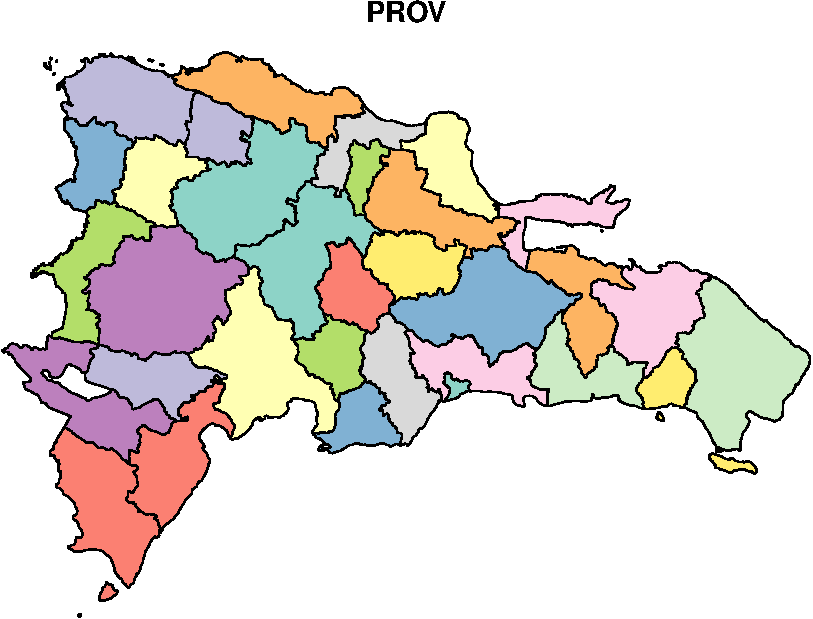
\includegraphics{proyecto_files/figure-latex/unnamed-chunk-4-1.pdf}

\begin{Shaded}
\begin{Highlighting}[]
\KeywordTok{st_crs}\NormalTok{(prep)}
\end{Highlighting}
\end{Shaded}

\begin{verbatim}
## Coordinate Reference System:
##   EPSG: 4326 
##   proj4string: "+proj=longlat +datum=WGS84 +no_defs"
\end{verbatim}

\begin{Shaded}
\begin{Highlighting}[]
\NormalTok{crsdestino <-}\StringTok{ }\DecValTok{32619}
\NormalTok{preputm <-}\StringTok{ }\NormalTok{prep }\OperatorTok\StringTok{ }\KeywordTok{st_transform}\NormalTok{(}\DataTypeTok{crs =}\NormalTok{ crsdestino)}
\NormalTok{preputm}
\end{Highlighting}
\end{Shaded}

\begin{verbatim}
## Simple feature collection with 25 features and 37 fields
## geometry type:  POINT
## dimension:      XY
## bbox:           xmin: 215264.1 ymin: 1999092 xmax: 566794.7 ymax: 2197035
## epsg (SRID):    32619
## proj4string:    +proj=utm +zone=19 +datum=WGS84 +units=m +no_defs
## First 10 features:
##            Estación  a1979  a1980  a1981  a1982  a1983  a1984  a1985
## 1          Barahona 1740.0 1053.6 1435.3  815.3 1183.0  584.1  997.8
## 2         Bayaguana 2794.3 1761.5 2412.4 1758.6 1857.1 1645.6 1928.3
## 3           Cabrera 2035.0 1276.8     NA 2136.9 1703.8 1888.7 1557.1
## 4         Constanza 1652.1 1166.9 1343.3  921.2  828.4     NA  892.8
## 5  Gaspar Hernández     NA 1443.8 2174.9 1844.1 1688.8 2208.8 1895.5
## 6       Hondo Valle 1823.6 1778.2 2203.7 1709.9 1841.3 1796.6 1309.5
## 7            Jimaní 1060.7  639.1  960.2  507.5  610.7  641.5  689.6
## 8          La Unión 1781.5 1630.6 2304.4 1413.1 1288.4 1499.4 1157.1
## 9           La Vega 1833.5 1304.3 1993.7 1483.2 1353.9 1550.1 1084.9
## 10     Las Américas 1958.4  958.7 1513.4  787.4  975.5  954.9 1398.2
##     a1986  a1987  a1988  a1989   a1990  a1991  a1992  a1993  a1994   a1995
## 1  1080.0 1423.9  704.7 1011.6 1075.20  983.1 1112.5  968.5 1622.4  956.00
## 2  2182.2 2273.5 1813.2 1730.6 1823.40 1850.3 1765.7 1606.2 1892.8 1360.10
## 3  1597.0 2059.7     NA 1176.9 1183.40  957.6     NA     NA     NA      NA
## 4   715.8  786.9  837.7  671.5  875.35     NA  858.6  858.6  900.7  839.40
## 5  2874.7 2360.8 1426.3 1214.2 1530.70     NA 1257.5 1345.3 1824.9 1665.45
## 6  1589.7 1778.8 1766.5 1722.8 1596.10 1088.4 1731.0 1887.0 1772.0 1288.30
## 7   802.4  648.9  521.0  680.7  880.00  311.6  809.2  472.9  840.2  909.00
## 8  1313.1 1786.5 1888.8 1222.8 1808.00 1250.4 1555.2 1484.8 1035.9  877.70
## 9  1767.1 1663.2 1934.9 1192.4 1664.40 1146.4 1565.6 1855.4 1455.7 1175.40
## 10 1419.0 1866.4 1620.5 1151.7      NA  997.0     NA     NA     NA 1017.50
##      a1996   a1997  a1998  a1999  a2000  a2001  a2002   a2003  a2004
## 1   965.65  662.60  684.6  662.7  600.0  600.0  997.6  942.60  972.6
## 2  1867.70 1618.60 2156.6 1712.5 1868.5 1796.1 1658.0 2117.30 1554.2
## 3       NA      NA     NA     NA 1538.6 1852.9  946.9 1810.95 2053.3
## 4  1167.30  525.10 1492.7 1077.8  951.3  787.1  959.2 1084.10  985.9
## 5  2656.80  984.80 2147.9 1791.9 1716.9 2178.8 1093.4 2058.50 1906.8
## 6  1447.90  912.65 1813.9 1762.2 2285.9 1604.3 1477.4 1628.10 1617.7
## 7   816.20  358.20  824.1 1037.0  833.9  488.4  510.1  656.70  866.9
## 8  1980.50  554.20 1744.1 1314.3 1148.5 1360.5  972.1 1802.00 2550.1
## 9  1772.50 1018.80 1549.6 1817.9 1368.6 1522.0 1200.7 2290.60 1825.7
## 10 1019.60  651.20 1218.6 1125.9  809.7  747.6  933.4 1083.60 1338.9
##      a2005   a2006   a2007   a2008  a2009  a2010  a2011  a2012  a2013
## 1  1274.60 1118.40 1531.30 1136.80  583.3 1036.3 1280.2 1726.3  576.2
## 2  2102.80 2097.10 2137.60 1831.20 1607.9 1881.6 1849.9 2350.8 2108.0
## 3  1451.10 1957.90      NA      NA     NA 2411.4 1920.1 2821.3     NA
## 4  1245.20 1162.20 1661.40 1072.90  902.8 1024.5 1008.2 1188.1 1016.3
## 5  2001.85 1992.00 3282.65 1866.30 2386.1 2639.2 1727.2 2524.0 1448.2
## 6  1554.65 1487.15 1487.15 1399.15 1461.9 2005.6 1309.0 1736.8 1390.2
## 7   929.30  963.90 1084.00  751.10  694.9  807.1  879.5 1037.3  292.9
## 8  2034.30 2106.60 2764.80 1536.30 1605.8 2255.6 1719.2 2484.3 1299.2
## 9  1245.20 1162.20 1661.40 1072.90 2867.4 1486.4 1434.1 2204.7 1227.0
## 10 1744.60 1141.70 1457.50 1718.40 1369.1 2422.4 1885.5 1658.7 1039.6
##     a2014                     geom
## 1   845.9 POINT (277900.2 2013585)
## 2  1505.6 POINT (433242.1 2073284)
## 3  1975.6   POINT (405636 2171119)
## 4   764.1 POINT (320947.7 2090623)
## 5  1928.7 POINT (363678.2 2169619)
## 6   908.9 POINT (215264.1 2071669)
## 7   502.0 POINT (221953.7 2045651)
## 8  1741.5 POINT (337592.1 2184559)
## 9  1812.5 POINT (338847.1 2125548)
## 10  909.4 POINT (429562.7 2038222)
\end{verbatim}

\begin{Shaded}
\begin{Highlighting}[]
\CommentTok{#Estadísticos Básicos del año 1994.}
\KeywordTok{nrow}\NormalTok{(preputm)}
\end{Highlighting}
\end{Shaded}

\begin{verbatim}
## [1] 25
\end{verbatim}

\begin{Shaded}
\begin{Highlighting}[]
\KeywordTok{summary}\NormalTok{(preputm}\OperatorTok{$}\NormalTok{a1994)}
\end{Highlighting}
\end{Shaded}

\begin{verbatim}
##    Min. 1st Qu.  Median    Mean 3rd Qu.    Max.    NA's 
##   650.0   967.1  1219.5  1326.2  1782.5  1933.7       2
\end{verbatim}

\begin{Shaded}
\begin{Highlighting}[]
\KeywordTok{hist}\NormalTok{(preputm}\OperatorTok{$}\NormalTok{a1994)}
\end{Highlighting}
\end{Shaded}

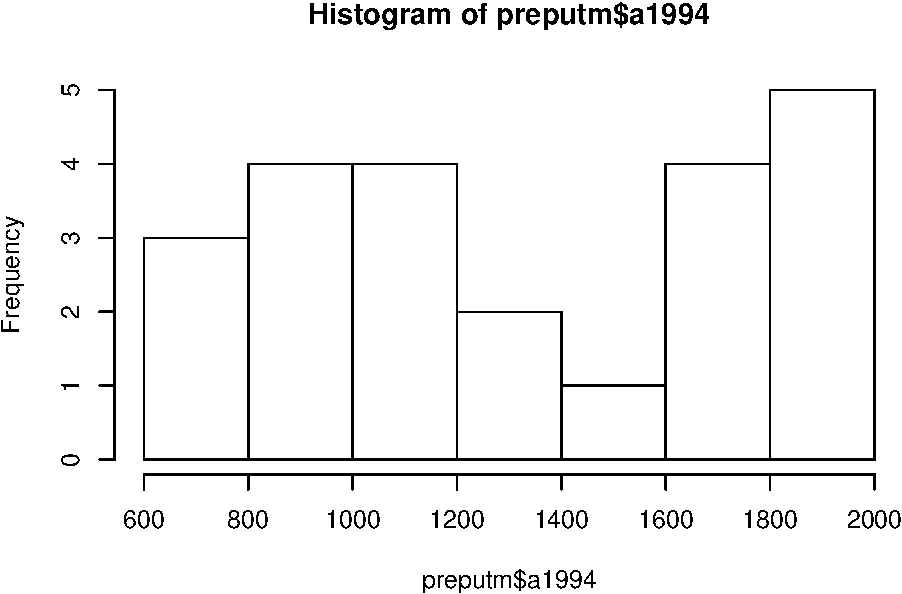
\includegraphics{proyecto_files/figure-latex/unnamed-chunk-4-2.pdf}

\begin{Shaded}
\begin{Highlighting}[]
\KeywordTok{hist}\NormalTok{(}\KeywordTok{log}\NormalTok{(preputm}\OperatorTok{$}\NormalTok{a1994))}
\end{Highlighting}
\end{Shaded}

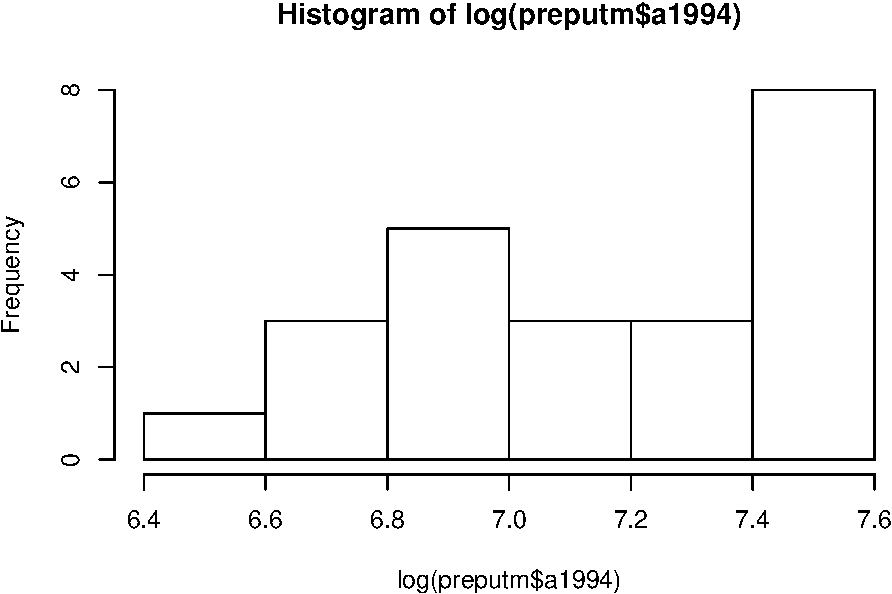
\includegraphics{proyecto_files/figure-latex/unnamed-chunk-4-3.pdf}

\begin{Shaded}
\begin{Highlighting}[]
\KeywordTok{shapiro.test}\NormalTok{(preputm}\OperatorTok{$}\NormalTok{a1994)}
\end{Highlighting}
\end{Shaded}

\begin{verbatim}
## 
##  Shapiro-Wilk normality test
## 
## data:  preputm$a1994
## W = 0.9062, p-value = 0.03399
\end{verbatim}

\begin{Shaded}
\begin{Highlighting}[]
\KeywordTok{shapiro.test}\NormalTok{(}\KeywordTok{log}\NormalTok{(prep}\OperatorTok{$}\NormalTok{a1994))}
\end{Highlighting}
\end{Shaded}

\begin{verbatim}
## 
##  Shapiro-Wilk normality test
## 
## data:  log(prep$a1994)
## W = 0.91635, p-value = 0.05567
\end{verbatim}

\begin{Shaded}
\begin{Highlighting}[]
\NormalTok{prep1994 <-}\StringTok{ }\KeywordTok{na.omit}\NormalTok{(preputm[,}\KeywordTok{c}\NormalTok{(}\StringTok{'Estación', '}\NormalTok{a1994}\StringTok{')])}
\StringTok{prep1994$a1994log <- log(prep1994$a1994)}
\StringTok{prep1994}
\end{Highlighting}
\end{Shaded}

\begin{verbatim}
## Simple feature collection with 23 features and 3 fields
## geometry type:  POINT
## dimension:      XY
## bbox:           xmin: 215264.1 ymin: 1999092 xmax: 566794.7 ymax: 2197035
## epsg (SRID):    32619
## proj4string:    +proj=utm +zone=19 +datum=WGS84 +units=m +no_defs
## First 10 features:
##            Estación   a1994                     geom a1994log
## 1          Barahona 1622.40 POINT (277900.2 2013585) 7.391662
## 2         Bayaguana 1892.80 POINT (433242.1 2073284) 7.545812
## 4         Constanza  900.70 POINT (320947.7 2090623) 6.803172
## 5  Gaspar Hernández 1824.90 POINT (363678.2 2169619) 7.509280
## 6       Hondo Valle 1772.00 POINT (215264.1 2071669) 7.479864
## 7            Jimaní  840.20 POINT (221953.7 2045651) 6.733640
## 8          La Unión 1035.90 POINT (337592.1 2184559) 6.943026
## 9           La Vega 1455.70 POINT (338847.1 2125548) 7.283242
## 11             Moca 1182.10 POINT (342475.8 2143891) 7.075048
## 12     Monte Cristi  650.05 POINT (224239.3 2197035) 6.477049
\end{verbatim}

\begin{Shaded}
\begin{Highlighting}[]
\CommentTok{#Ilustraciónde los Observatorios correspondiente  a la precipitación}
\KeywordTok{ggplot}\NormalTok{() }\OperatorTok{+}
\StringTok{  }\KeywordTok{geom_sf}\NormalTok{(}\DataTypeTok{data =}\NormalTok{ prov, }\DataTypeTok{fill =} \StringTok{'white'}\NormalTok{) }\OperatorTok{+}
\StringTok{  }\KeywordTok{geom_sf}\NormalTok{(}\DataTypeTok{data =}\NormalTok{ prep1994, }\KeywordTok{aes}\NormalTok{(}\DataTypeTok{col =}\NormalTok{ a1994log), }\DataTypeTok{size =} \DecValTok{6}\NormalTok{) }\OperatorTok{+}
\StringTok{  }\KeywordTok{scale_colour_gradient}\NormalTok{(}\DataTypeTok{low=}\StringTok{"#deebf7"}\NormalTok{, }\DataTypeTok{high=}\StringTok{"#3182bd"}\NormalTok{) }\OperatorTok{+}
\StringTok{  }\KeywordTok{geom_sf_text}\NormalTok{(}\DataTypeTok{data =}\NormalTok{ prov, }\KeywordTok{aes}\NormalTok{(}\DataTypeTok{label=}\NormalTok{TOPONIMIA), }\DataTypeTok{check_overlap =}\NormalTok{ T, }\DataTypeTok{size =} \DecValTok{2}\NormalTok{) }\OperatorTok{+}
\StringTok{  }\KeywordTok{geom_sf_text}\NormalTok{(}\DataTypeTok{data =}\NormalTok{ prep1994, }\KeywordTok{aes}\NormalTok{(}\DataTypeTok{label=}\NormalTok{Estación), }\DataTypeTok{check_overlap =}\NormalTok{ T, }\DataTypeTok{size =} \FloatTok{1.5}\NormalTok{) }\OperatorTok{+}
\StringTok{  }\KeywordTok{theme_bw}\NormalTok{()}
\end{Highlighting}
\end{Shaded}

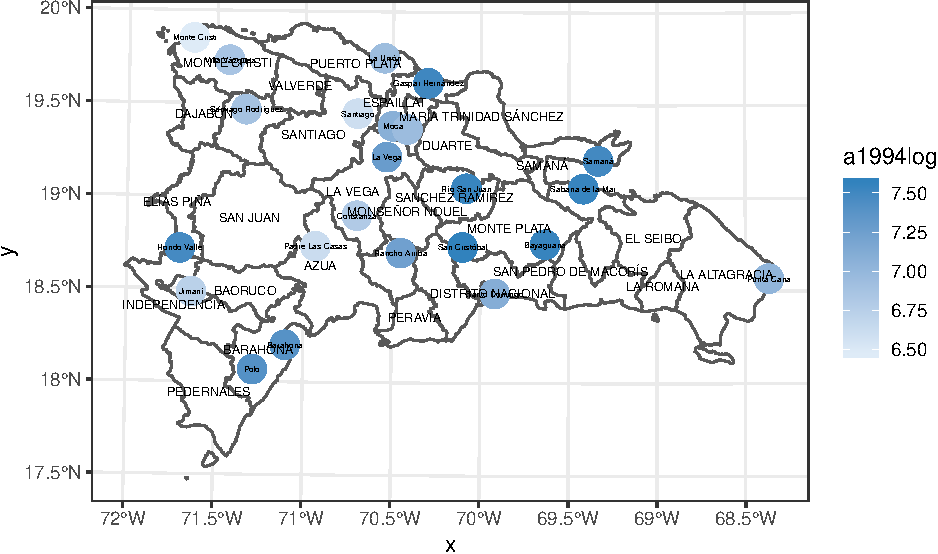
\includegraphics{proyecto_files/figure-latex/unnamed-chunk-4-4.pdf}

\begin{Shaded}
\begin{Highlighting}[]
\CommentTok{#Viariograma Muestral}
\NormalTok{v1994 <-}\StringTok{ }\KeywordTok{variogram}\NormalTok{(a1994log}\OperatorTok{~}\DecValTok{1}\NormalTok{, prep1994)}
\NormalTok{v1994}
\end{Highlighting}
\end{Shaded}

\begin{verbatim}
##    np       dist       gamma dir.hor dir.ver   id
## 1   1   8896.559 0.007944882       0       0 var1
## 2   7  22355.182 0.077600672       0       0 var1
## 3  10  32118.137 0.092137842       0       0 var1
## 4   7  40140.925 0.047553298       0       0 var1
## 5   7  50078.452 0.131083955       0       0 var1
## 6  12  58814.056 0.067784634       0       0 var1
## 7   9  67157.152 0.130336228       0       0 var1
## 8   7  77916.592 0.098909157       0       0 var1
## 9  18  85575.296 0.115075028       0       0 var1
## 10 11  93434.242 0.102473601       0       0 var1
## 11  9 103937.517 0.114591447       0       0 var1
## 12 19 112257.676 0.090228623       0       0 var1
## 13 15 120286.239 0.094253570       0       0 var1
## 14 11 128864.926 0.133333296       0       0 var1
\end{verbatim}

\begin{Shaded}
\begin{Highlighting}[]
\KeywordTok{plot}\NormalTok{(v1994, }\DataTypeTok{plot.numbers =}\NormalTok{ T)}
\end{Highlighting}
\end{Shaded}

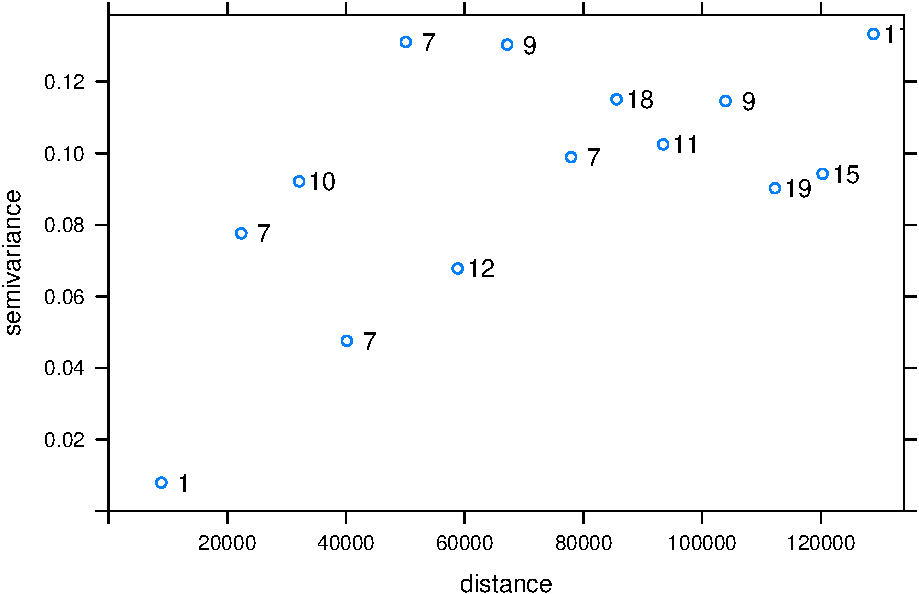
\includegraphics{proyecto_files/figure-latex/unnamed-chunk-4-5.pdf}

\begin{Shaded}
\begin{Highlighting}[]
\CommentTok{#Generamos varios variogramas con la finalidad de elegir el que utilizaremos en la interpolación del Kriging Ordinario.}
\NormalTok{v1994_m <-}\StringTok{ }\KeywordTok{fit.variogram}\NormalTok{(v1994, }\KeywordTok{vgm}\NormalTok{(}\DataTypeTok{model =} \StringTok{"Sph"}\NormalTok{, }\DataTypeTok{range =} \DecValTok{50000}\NormalTok{))}
\NormalTok{v1994_m}
\end{Highlighting}
\end{Shaded}

\begin{verbatim}
##   model     psill    range
## 1   Sph 0.1009413 49767.72
\end{verbatim}

\begin{Shaded}
\begin{Highlighting}[]
\KeywordTok{plot}\NormalTok{(v1994, v1994_m, }\DataTypeTok{plot.numbers =}\NormalTok{ T)}
\end{Highlighting}
\end{Shaded}

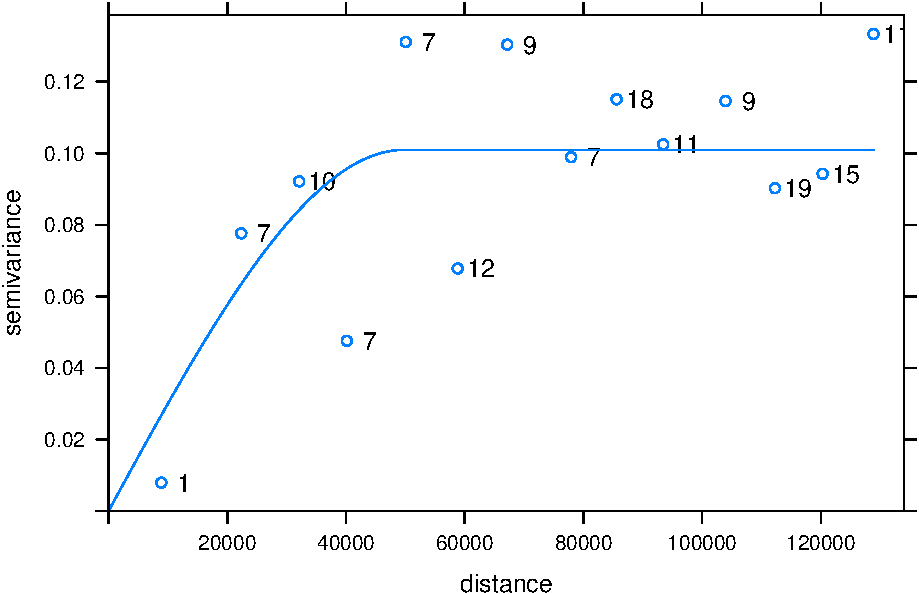
\includegraphics{proyecto_files/figure-latex/unnamed-chunk-4-6.pdf}

\begin{Shaded}
\begin{Highlighting}[]
\NormalTok{v1994_m2 <-}\StringTok{ }\KeywordTok{fit.variogram}\NormalTok{(v1994, }\KeywordTok{vgm}\NormalTok{(}\DataTypeTok{model =} \StringTok{"Exp"}\NormalTok{, }\DataTypeTok{range =} \DecValTok{50000}\NormalTok{))}
\NormalTok{v1994_m2}
\end{Highlighting}
\end{Shaded}

\begin{verbatim}
##   model     psill    range
## 1   Exp 0.1113154 26274.06
\end{verbatim}

\begin{Shaded}
\begin{Highlighting}[]
\KeywordTok{plot}\NormalTok{(v1994, v1994_m2, }\DataTypeTok{plot.numbers =}\NormalTok{ T)}
\end{Highlighting}
\end{Shaded}

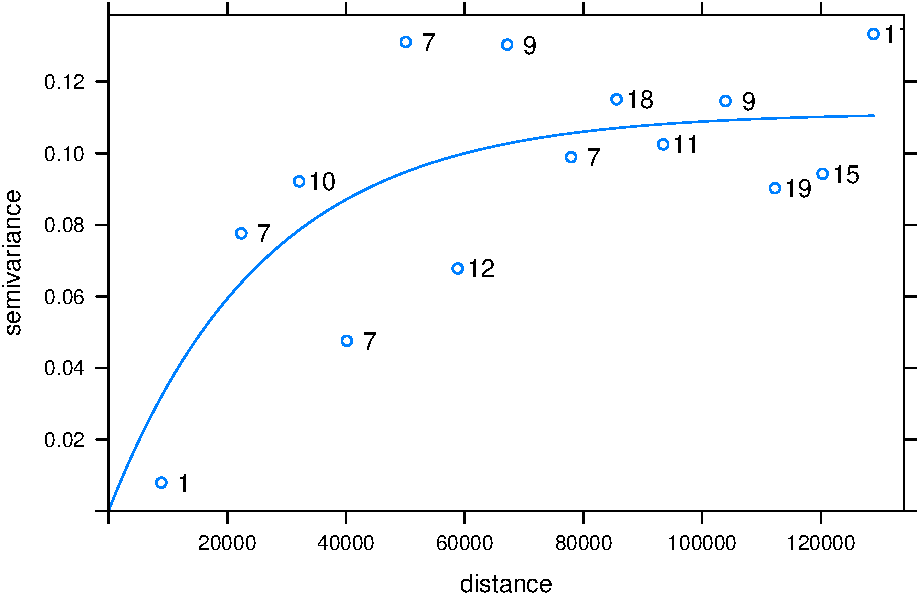
\includegraphics{proyecto_files/figure-latex/unnamed-chunk-4-7.pdf}

\begin{Shaded}
\begin{Highlighting}[]
\NormalTok{v1994_m3 <-}\StringTok{ }\KeywordTok{fit.variogram}\NormalTok{(v1994, }\KeywordTok{vgm}\NormalTok{(}\DataTypeTok{model =} \StringTok{"Gau"}\NormalTok{, }\DataTypeTok{range =} \DecValTok{50000}\NormalTok{))}
\NormalTok{v1994_m3}
\end{Highlighting}
\end{Shaded}

\begin{verbatim}
##   model      psill    range
## 1   Gau 0.09862521 20674.73
\end{verbatim}

\begin{Shaded}
\begin{Highlighting}[]
\KeywordTok{plot}\NormalTok{(v1994, v1994_m3, }\DataTypeTok{plot.numbers =}\NormalTok{ T)}
\end{Highlighting}
\end{Shaded}

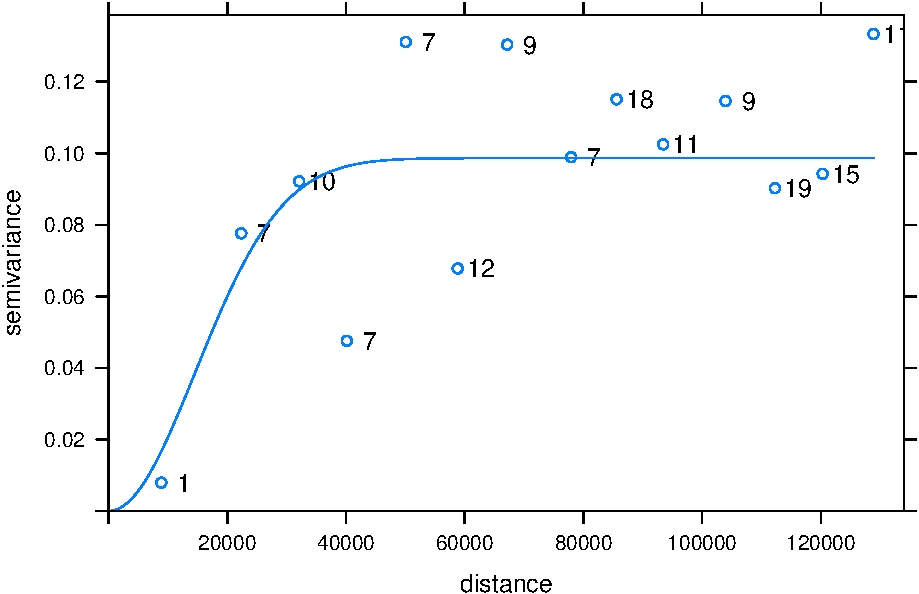
\includegraphics{proyecto_files/figure-latex/unnamed-chunk-4-8.pdf}

\begin{Shaded}
\begin{Highlighting}[]
\KeywordTok{attr}\NormalTok{(v1994_m, }\StringTok{'SSErr'}\NormalTok{) }
\end{Highlighting}
\end{Shaded}

\begin{verbatim}
## [1] 2.759794e-11
\end{verbatim}

\begin{Shaded}
\begin{Highlighting}[]
\KeywordTok{attr}\NormalTok{(v1994_m2, }\StringTok{'SSErr'}\NormalTok{)}
\end{Highlighting}
\end{Shaded}

\begin{verbatim}
## [1] 2.872536e-11
\end{verbatim}

\begin{Shaded}
\begin{Highlighting}[]
\KeywordTok{attr}\NormalTok{(v1994_m3, }\StringTok{'SSErr'}\NormalTok{)}\CommentTok{#Elegimos este}
\end{Highlighting}
\end{Shaded}

\begin{verbatim}
## [1] 2.27658e-11
\end{verbatim}

\begin{Shaded}
\begin{Highlighting}[]
\NormalTok{grd <-}\StringTok{ }\KeywordTok{st_bbox}\NormalTok{(prov) }\OperatorTok
\StringTok{  }\KeywordTok{st_as_stars}\NormalTok{(}\DataTypeTok{dx =} \DecValTok{3000}\NormalTok{) }\OperatorTok\StringTok{ }\CommentTok{# 3000 metros=3km de resolución espacial}
\StringTok{  }\KeywordTok{st_set_crs}\NormalTok{(crsdestino) }\OperatorTok
\StringTok{  }\KeywordTok{st_crop}\NormalTok{(prov)}
\NormalTok{grd}
\end{Highlighting}
\end{Shaded}

\begin{verbatim}
## stars object with 2 dimensions and 1 attribute
## attribute(s):
##     values     
##  Min.   :0     
##  1st Qu.:0     
##  Median :0     
##  Mean   :0     
##  3rd Qu.:0     
##  Max.   :0     
##  NA's   :6501  
## dimension(s):
##   from  to  offset delta                       refsys point values    
## x    1 130  182216  3000 +proj=utm +zone=19 +datum...    NA   NULL [x]
## y    1  91 2205216 -3000 +proj=utm +zone=19 +datum...    NA   NULL [y]
\end{verbatim}

\begin{Shaded}
\begin{Highlighting}[]
\KeywordTok{plot}\NormalTok{(grd)}
\end{Highlighting}
\end{Shaded}

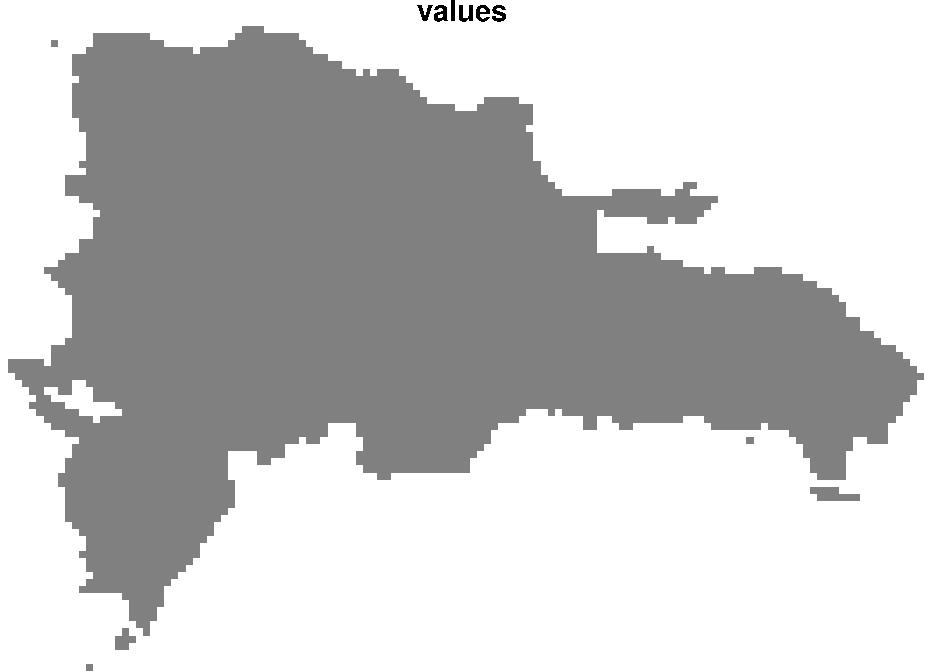
\includegraphics{proyecto_files/figure-latex/unnamed-chunk-4-9.pdf}

\begin{Shaded}
\begin{Highlighting}[]
\CommentTok{#Generamos una cuadrícula para RD y sobre ella realizamos el Kriging ordinario.}
\NormalTok{k <-}\StringTok{ }\KeywordTok{krige}\NormalTok{(}\DataTypeTok{formula =}\NormalTok{ a1994log}\OperatorTok{~}\DecValTok{1}\NormalTok{, }\DataTypeTok{locations =}\NormalTok{ prep1994, }\DataTypeTok{newdata =}\NormalTok{ grd, }\DataTypeTok{model =}\NormalTok{ v1994_m3)}
\end{Highlighting}
\end{Shaded}

\begin{verbatim}
## [using ordinary kriging]
\end{verbatim}

\begin{Shaded}
\begin{Highlighting}[]
\NormalTok{k}
\end{Highlighting}
\end{Shaded}

\begin{verbatim}
## stars object with 2 dimensions and 2 attributes
## attribute(s):
##    var1.pred       var1.var     
##  Min.   :6.479   Min.   :0.000  
##  1st Qu.:7.064   1st Qu.:0.057  
##  Median :7.130   Median :0.092  
##  Mean   :7.131   Mean   :0.077  
##  3rd Qu.:7.209   3rd Qu.:0.103  
##  Max.   :7.572   Max.   :0.104  
##  NA's   :6501    NA's   :6501   
## dimension(s):
##   from  to  offset delta                       refsys point values    
## x    1 130  182216  3000 +proj=utm +zone=19 +datum...    NA   NULL [x]
## y    1  91 2205216 -3000 +proj=utm +zone=19 +datum...    NA   NULL [y]
\end{verbatim}

\begin{Shaded}
\begin{Highlighting}[]
\KeywordTok{plot}\NormalTok{(k)}
\end{Highlighting}
\end{Shaded}

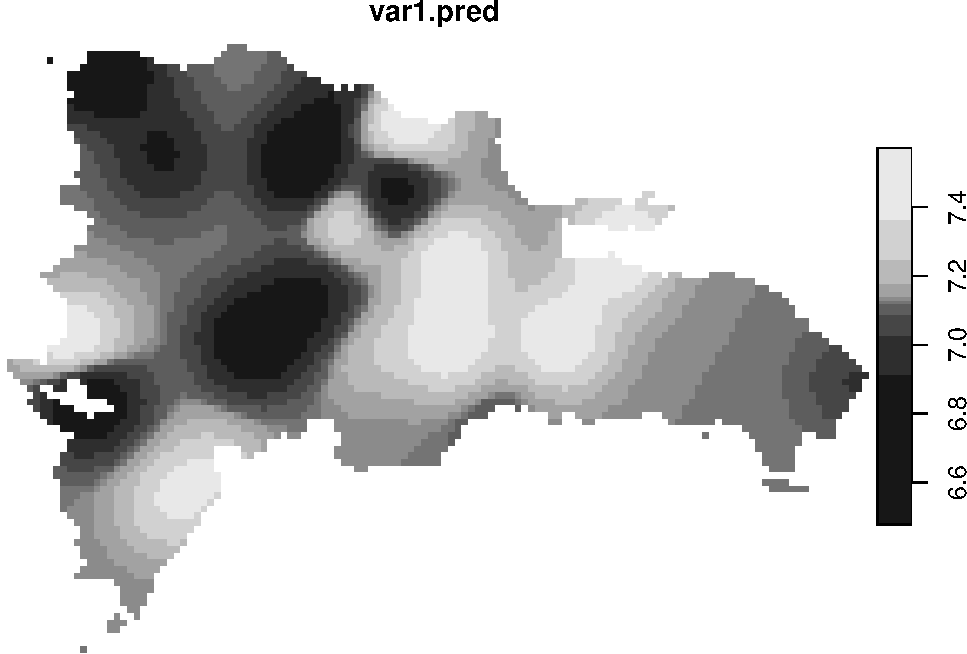
\includegraphics{proyecto_files/figure-latex/unnamed-chunk-4-10.pdf}

\begin{Shaded}
\begin{Highlighting}[]
\KeywordTok{ggplot}\NormalTok{() }\OperatorTok{+}
\StringTok{  }\KeywordTok{geom_stars}\NormalTok{(}\DataTypeTok{data =}\NormalTok{ k, }\KeywordTok{aes}\NormalTok{(}\DataTypeTok{fill =}\NormalTok{ var1.pred, }\DataTypeTok{x =}\NormalTok{ x, }\DataTypeTok{y =}\NormalTok{ y)) }\OperatorTok{+}\StringTok{ }
\StringTok{  }\KeywordTok{scale_fill_gradient}\NormalTok{(}\DataTypeTok{low=}\StringTok{"#deebf7"}\NormalTok{, }\DataTypeTok{high=}\StringTok{"#3182bd"}\NormalTok{) }\OperatorTok{+}
\StringTok{  }\KeywordTok{geom_sf}\NormalTok{(}\DataTypeTok{data =} \KeywordTok{st_cast}\NormalTok{(prov, }\StringTok{"MULTILINESTRING"}\NormalTok{)) }\OperatorTok{+}
\StringTok{  }\KeywordTok{geom_sf}\NormalTok{(}\DataTypeTok{data =}\NormalTok{ prep1994) }\OperatorTok{+}
\StringTok{  }\KeywordTok{geom_sf_text}\NormalTok{(}\DataTypeTok{data =}\NormalTok{ prov, }\KeywordTok{aes}\NormalTok{(}\DataTypeTok{label=}\NormalTok{TOPONIMIA), }\DataTypeTok{check_overlap =}\NormalTok{ T, }\DataTypeTok{size =} \DecValTok{2}\NormalTok{) }\OperatorTok{+}
\StringTok{  }\KeywordTok{theme_bw}\NormalTok{()}
\end{Highlighting}
\end{Shaded}

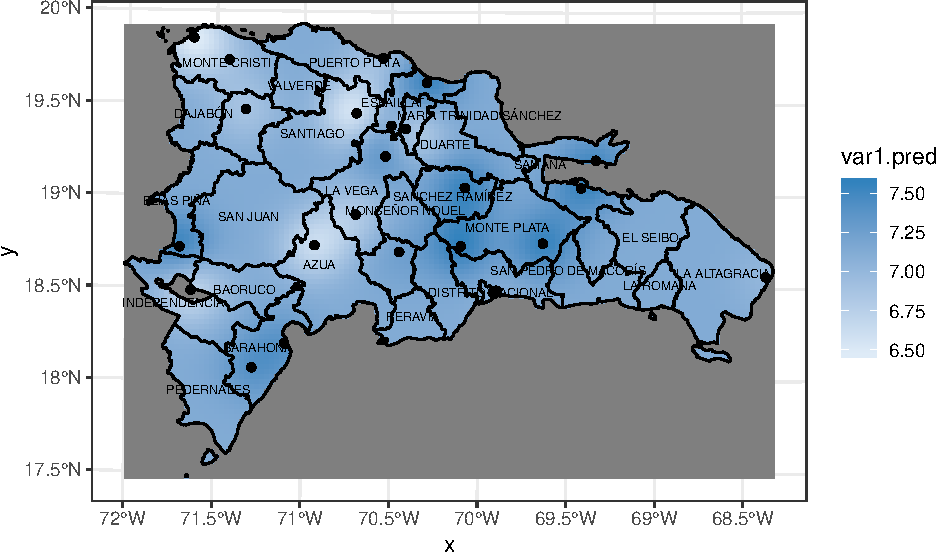
\includegraphics{proyecto_files/figure-latex/unnamed-chunk-4-11.pdf}

\begin{Shaded}
\begin{Highlighting}[]
\KeywordTok{ggplot}\NormalTok{() }\OperatorTok{+}
\StringTok{  }\KeywordTok{geom_stars}\NormalTok{(}\DataTypeTok{data =} \KeywordTok{exp}\NormalTok{(k), }\KeywordTok{aes}\NormalTok{(}\DataTypeTok{fill =}\NormalTok{ var1.pred, }\DataTypeTok{x =}\NormalTok{ x, }\DataTypeTok{y =}\NormalTok{ y)) }\OperatorTok{+}\StringTok{ }
\StringTok{  }\KeywordTok{scale_fill_gradient}\NormalTok{(}\DataTypeTok{low=}\StringTok{"#deebf7"}\NormalTok{, }\DataTypeTok{high=}\StringTok{"#3182bd"}\NormalTok{, }\DataTypeTok{trans =} \StringTok{'log10'}\NormalTok{) }\OperatorTok{+}
\StringTok{  }\KeywordTok{geom_sf}\NormalTok{(}\DataTypeTok{data =} \KeywordTok{st_cast}\NormalTok{(prov, }\StringTok{"MULTILINESTRING"}\NormalTok{)) }\OperatorTok{+}
\StringTok{  }\KeywordTok{geom_sf}\NormalTok{(}\DataTypeTok{data =}\NormalTok{ prep1994) }\OperatorTok{+}
\StringTok{  }\KeywordTok{geom_sf_text}\NormalTok{(}\DataTypeTok{data =}\NormalTok{ prov, }\KeywordTok{aes}\NormalTok{(}\DataTypeTok{label=}\NormalTok{TOPONIMIA), }\DataTypeTok{check_overlap =}\NormalTok{ T, }\DataTypeTok{size =} \DecValTok{2}\NormalTok{) }\OperatorTok{+}
\StringTok{  }\KeywordTok{theme_bw}\NormalTok{()}
\end{Highlighting}
\end{Shaded}

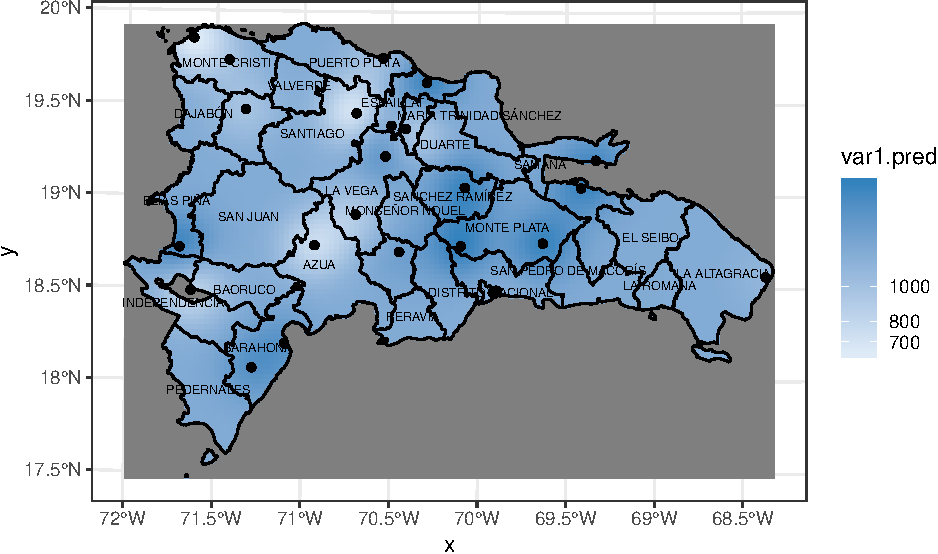
\includegraphics{proyecto_files/figure-latex/unnamed-chunk-4-12.pdf} \#
Referencias

Análisis espacial con R: Usa R como un Sistema de Información
Geográfica, de JEAN-FRANCOIS MAS.

\url{http://onamet.gob.do/index.php/sobre-nosotros/quienes-somos}

\url{http://www.scielo.org.mx/scielo.php?script=sci_arttext\&pid=S1405-31952009000100001}

\url{https://www.sgapeio.es/INFORMEST/VICongreso/artigos/sesion1_04.pdf}

\url{https://prezi.com/l7zplkrgogbo/proyecto-de-investigacio-sobre-precipitacion-pluvial/}

\url{https://www.academia.edu/17328936/CARACTERISTICAS_VARIOGRAMA}

\url{https://acolita.com/geoestadistica-interpolacion-con-kriging/}

\url{https://www.monografias.com/docs114/principios-variogramas/principios-variogramas3.shtml}

\url{https://volaya.github.io/libro-sig/chapters/Estadistica_espacial.html}




\newpage
\singlespacing 
\end{document}
